\documentclass{standalone}
\usepackage{tikz}
\usetikzlibrary{patterns, positioning}
\usepackage[sfdefault]{ClearSans} %% option 'sfdefault' activates Clear Sans as the default text font
\usepackage[T1]{fontenc}

\begin{document}
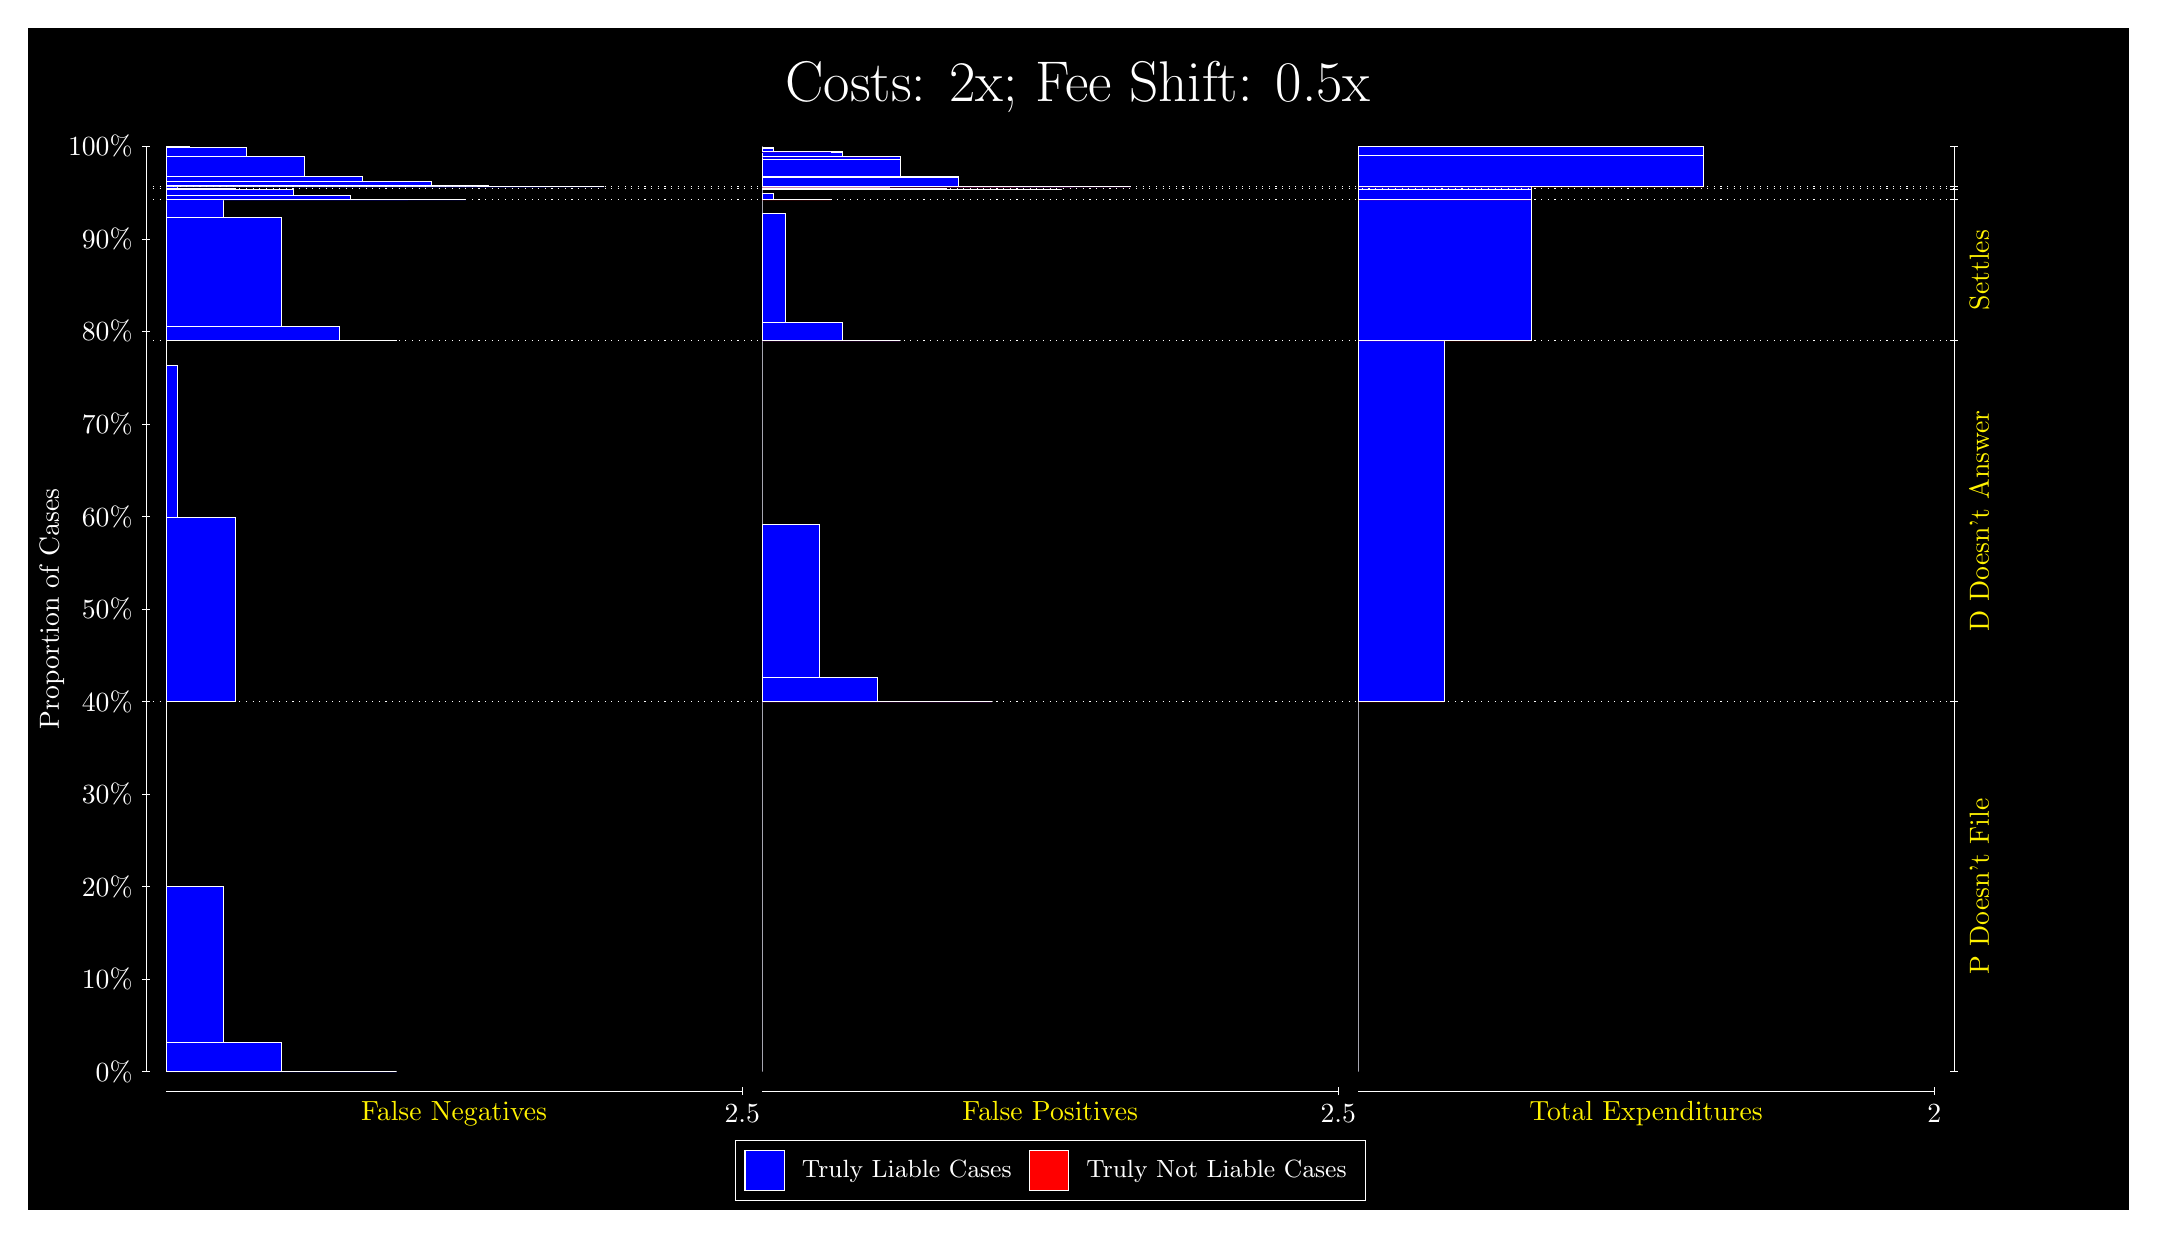
\begin{tikzpicture}
\draw[fill=black] (0,0) rectangle (26.667,15);
\draw[text=white] (0,13.5) rectangle (26.667,15) node[midway] {\huge Costs: 2x; Fee Shift: 0.5x};
\draw[white, very thin] (1.5,1.75) -- (1.5,13.5);
\node[rotate=90, text=white, anchor=center] at (0.3, 7.625) {Proportion of Cases};
\draw[white, very thin] (1.45,1.75) -- (1.55,1.75);
\node[text=white, anchor=east] at (1.45, 1.75) {0\%};
\draw[white, very thin] (1.45,2.925) -- (1.55,2.925);
\node[text=white, anchor=east] at (1.45, 2.925) {10\%};
\draw[white, very thin] (1.45,4.1) -- (1.55,4.1);
\node[text=white, anchor=east] at (1.45, 4.1) {20\%};
\draw[white, very thin] (1.45,5.275) -- (1.55,5.275);
\node[text=white, anchor=east] at (1.45, 5.275) {30\%};
\draw[white, very thin] (1.45,6.45) -- (1.55,6.45);
\node[text=white, anchor=east] at (1.45, 6.45) {40\%};
\draw[white, very thin] (1.45,7.625) -- (1.55,7.625);
\node[text=white, anchor=east] at (1.45, 7.625) {50\%};
\draw[white, very thin] (1.45,8.8) -- (1.55,8.8);
\node[text=white, anchor=east] at (1.45, 8.8) {60\%};
\draw[white, very thin] (1.45,9.975) -- (1.55,9.975);
\node[text=white, anchor=east] at (1.45, 9.975) {70\%};
\draw[white, very thin] (1.45,11.15) -- (1.55,11.15);
\node[text=white, anchor=east] at (1.45, 11.15) {80\%};
\draw[white, very thin] (1.45,12.325) -- (1.55,12.325);
\node[text=white, anchor=east] at (1.45, 12.325) {90\%};
\draw[white, very thin] (1.45,13.5) -- (1.55,13.5);
\node[text=white, anchor=east] at (1.45, 13.5) {100\%};

\draw[white, very thin] (24.457,1.75) -- (24.457,13.5);
\draw[white, very thin] (24.407,1.75) -- (24.507,1.75);
\node[anchor=west] at (24.407, 1.75) {};
\draw[white, very thin] (24.407,6.4489) -- (24.507,6.4489);
\node[anchor=west] at (24.407, 6.4489) {};
\draw[white, very thin] (24.407,11.033) -- (24.507,11.033);
\node[anchor=west] at (24.407, 11.033) {};
\draw[white, very thin] (24.407,12.824) -- (24.507,12.824);
\node[anchor=west] at (24.407, 12.824) {};
\draw[white, very thin] (24.407,12.96) -- (24.507,12.96);
\node[anchor=west] at (24.407, 12.96) {};
\draw[white, very thin] (24.407,12.989) -- (24.507,12.989);
\node[anchor=west] at (24.407, 12.989) {};
\draw[white, very thin] (24.407,13.5) -- (24.507,13.5);
\node[anchor=west] at (24.407, 13.5) {};

\draw[white, very thin, fill=blue] (1.75,1.75) rectangle (4.6775,1.75);
\draw[white, very thin, fill=blue] (1.75,1.75) rectangle (3.9457,1.7532);
\draw[white, very thin, fill=blue] (1.75,1.7532) rectangle (3.2138,2.126);
\draw[white, very thin, fill=blue] (1.75,2.126) rectangle (2.4819,4.1027);
\draw[white, very thin, fill=red] (1.75,4.1027) rectangle (1.75,4.1027);
\draw[white, very thin, fill=blue] (1.75,4.1027) rectangle (1.75,6.4489);
\draw[white, very thin, fill=blue] (1.75,6.4489) rectangle (2.6283,8.7857);
\draw[white, very thin, fill=blue] (1.75,8.7857) rectangle (1.8964,10.725);
\draw[white, very thin, fill=red] (1.75,10.725) rectangle (1.75,10.725);
\draw[white, very thin, fill=blue] (1.75,10.725) rectangle (1.75,11.033);
\draw[white, very thin, fill=blue] (1.75,11.033) rectangle (4.6775,11.034);
\draw[white, very thin, fill=blue] (1.75,11.034) rectangle (3.9457,11.211);
\draw[white, very thin, fill=blue] (1.75,11.211) rectangle (3.2138,12.597);
\draw[white, very thin, fill=blue] (1.75,12.597) rectangle (2.4819,12.824);
\draw[white, very thin, fill=red] (1.75,12.824) rectangle (1.75,12.824);
\draw[white, very thin, fill=blue] (1.75,12.824) rectangle (1.75,12.824);
\draw[white, very thin, fill=blue] (1.75,12.824) rectangle (5.5558,12.824);
\draw[white, very thin, fill=blue] (1.75,12.824) rectangle (4.8239,12.824);
\draw[white, very thin, fill=blue] (1.75,12.824) rectangle (4.092,12.875);
\draw[white, very thin, fill=blue] (1.75,12.875) rectangle (3.3602,12.958);
\draw[white, very thin, fill=blue] (1.75,12.958) rectangle (2.6283,12.96);
\draw[white, very thin, fill=red] (1.75,12.96) rectangle (1.75,12.96);
\draw[white, very thin, fill=blue] (1.75,12.96) rectangle (2.6283,12.969);
\draw[white, very thin, fill=blue] (1.75,12.969) rectangle (1.8964,12.988);
\draw[white, very thin, fill=red] (1.75,12.988) rectangle (1.75,12.988);
\draw[white, very thin, fill=blue] (1.75,12.988) rectangle (1.75,12.989);
\draw[white, very thin, fill=blue] (1.75,12.989) rectangle (7.3123,12.989);
\draw[white, very thin, fill=blue] (1.75,12.989) rectangle (6.5805,12.989);
\draw[white, very thin, fill=blue] (1.75,12.989) rectangle (5.8486,12.999);
\draw[white, very thin, fill=blue] (1.75,12.999) rectangle (5.7022,12.999);
\draw[white, very thin, fill=blue] (1.75,12.999) rectangle (5.1167,13.054);
\draw[white, very thin, fill=blue] (1.75,13.054) rectangle (4.9703,13.054);
\draw[white, very thin, fill=blue] (1.75,13.054) rectangle (4.3848,13.056);
\draw[white, very thin, fill=blue] (1.75,13.056) rectangle (4.2384,13.119);
\draw[white, very thin, fill=blue] (1.75,13.119) rectangle (3.6529,13.119);
\draw[white, very thin, fill=blue] (1.75,13.119) rectangle (3.5065,13.375);
\draw[white, very thin, fill=blue] (1.75,13.375) rectangle (2.7746,13.493);
\draw[white, very thin, fill=blue] (1.75,13.493) rectangle (2.0428,13.5);
\draw[white, very thin, fill=red] (1.75,13.5) rectangle (1.75,13.5);
\draw[white, very thin, fill=blue] (1.75,13.5) rectangle (1.75,13.5);
\draw[white, very thin, fill=red] (9.3189,1.75) rectangle (9.3189,1.75);
\draw[white, very thin, fill=blue] (9.3189,1.75) rectangle (9.3189,6.4489);
\draw[white, very thin, fill=red] (9.3189,6.4489) rectangle (12.246,6.4489);
\draw[white, very thin, fill=blue] (9.3189,6.4489) rectangle (12.246,6.4489);
\draw[white, very thin, fill=blue] (9.3189,6.4489) rectangle (11.515,6.4494);
\draw[white, very thin, fill=blue] (9.3189,6.4494) rectangle (10.783,6.7565);
\draw[white, very thin, fill=blue] (9.3189,6.7565) rectangle (10.051,8.6961);
\draw[white, very thin, fill=blue] (9.3189,8.6961) rectangle (9.3189,11.033);
\draw[white, very thin, fill=red] (9.3189,11.033) rectangle (11.075,11.033);
\draw[white, very thin, fill=blue] (9.3189,11.033) rectangle (11.075,11.033);
\draw[white, very thin, fill=blue] (9.3189,11.033) rectangle (10.344,11.26);
\draw[white, very thin, fill=blue] (9.3189,11.26) rectangle (9.6116,12.646);
\draw[white, very thin, fill=blue] (9.3189,12.646) rectangle (9.3189,12.824);
\draw[white, very thin, fill=red] (9.3189,12.824) rectangle (10.197,12.824);
\draw[white, very thin, fill=blue] (9.3189,12.824) rectangle (10.197,12.826);
\draw[white, very thin, fill=blue] (9.3189,12.826) rectangle (9.4652,12.909);
\draw[white, very thin, fill=blue] (9.3189,12.909) rectangle (9.3189,12.96);
\draw[white, very thin, fill=red] (9.3189,12.96) rectangle (13.125,12.96);
\draw[white, very thin, fill=blue] (9.3189,12.96) rectangle (13.125,12.96);
\draw[white, very thin, fill=blue] (9.3189,12.96) rectangle (12.393,12.96);
\draw[white, very thin, fill=blue] (9.3189,12.96) rectangle (11.661,12.961);
\draw[white, very thin, fill=blue] (9.3189,12.961) rectangle (10.929,12.98);
\draw[white, very thin, fill=blue] (9.3189,12.98) rectangle (10.197,12.989);
\draw[white, very thin, fill=red] (9.3189,12.989) rectangle (14.003,12.989);
\draw[white, very thin, fill=blue] (9.3189,12.989) rectangle (14.003,12.989);
\draw[white, very thin, fill=red] (9.3189,12.989) rectangle (13.271,12.989);
\draw[white, very thin, fill=blue] (9.3189,12.989) rectangle (13.271,12.989);
\draw[white, very thin, fill=red] (9.3189,12.989) rectangle (12.539,12.989);
\draw[white, very thin, fill=blue] (9.3189,12.989) rectangle (12.539,12.996);
\draw[white, very thin, fill=blue] (9.3189,12.996) rectangle (11.807,13.113);
\draw[white, very thin, fill=red] (9.3189,13.113) rectangle (11.807,13.113);
\draw[white, very thin, fill=blue] (9.3189,13.113) rectangle (11.807,13.114);
\draw[white, very thin, fill=blue] (9.3189,13.114) rectangle (11.075,13.338);
\draw[white, very thin, fill=blue] (9.3189,13.338) rectangle (11.075,13.369);
\draw[white, very thin, fill=red] (9.3189,13.369) rectangle (10.929,13.369);
\draw[white, very thin, fill=blue] (9.3189,13.369) rectangle (10.929,13.369);
\draw[white, very thin, fill=blue] (9.3189,13.369) rectangle (10.344,13.42);
\draw[white, very thin, fill=blue] (9.3189,13.42) rectangle (10.344,13.433);
\draw[white, very thin, fill=blue] (9.3189,13.433) rectangle (10.197,13.434);
\draw[white, very thin, fill=red] (9.3189,13.434) rectangle (10.197,13.434);
\draw[white, very thin, fill=blue] (9.3189,13.434) rectangle (10.197,13.435);
\draw[white, very thin, fill=blue] (9.3189,13.435) rectangle (9.6116,13.435);
\draw[white, very thin, fill=blue] (9.3189,13.435) rectangle (9.6116,13.435);
\draw[white, very thin, fill=blue] (9.3189,13.435) rectangle (9.4652,13.475);
\draw[white, very thin, fill=blue] (9.3189,13.475) rectangle (9.4652,13.49);
\draw[white, very thin, fill=blue] (9.3189,13.49) rectangle (9.3189,13.5);
\draw[white, very thin, fill=red] (16.888,1.75) rectangle (16.888,1.75);
\draw[white, very thin, fill=blue] (16.888,1.75) rectangle (16.888,6.4489);
\draw[white, very thin, fill=red] (16.888,6.4489) rectangle (17.986,6.4489);
\draw[white, very thin, fill=blue] (16.888,6.4489) rectangle (17.986,11.033);
\draw[white, very thin, fill=red] (16.888,11.033) rectangle (19.083,11.033);
\draw[white, very thin, fill=blue] (16.888,11.033) rectangle (19.083,12.824);
\draw[white, very thin, fill=red] (16.888,12.824) rectangle (19.083,12.824);
\draw[white, very thin, fill=blue] (16.888,12.824) rectangle (19.083,12.96);
\draw[white, very thin, fill=red] (16.888,12.96) rectangle (19.083,12.96);
\draw[white, very thin, fill=blue] (16.888,12.96) rectangle (19.083,12.989);
\draw[white, very thin, fill=red] (16.888,12.989) rectangle (21.279,12.989);
\draw[white, very thin, fill=blue] (16.888,12.989) rectangle (21.279,13.388);
\draw[white, very thin, fill=red] (16.888,13.388) rectangle (21.279,13.388);
\draw[white, very thin, fill=blue] (16.888,13.388) rectangle (21.279,13.5);
\draw[white, dotted] (1.5,6.4489) -- (24.457,6.4489);
\draw[white, dotted] (1.5,11.033) -- (24.457,11.033);
\draw[white, dotted] (1.5,12.824) -- (24.457,12.824);
\draw[white, dotted] (1.5,12.96) -- (24.457,12.96);
\draw[white, dotted] (1.5,12.989) -- (24.457,12.989);
\draw[white, very thin] (1.75,1.5) -- (9.0689,1.5);
\node[text=yellow, anchor=north] at (5.4094, 1.5) {False Negatives};
\draw[white, very thin] (9.0689,1.45) -- (9.0689,1.55);
\node[text=white, anchor=north] at (9.0689, 1.45) {2.5};

\draw[white, very thin] (9.3189,1.5) -- (16.638,1.5);
\node[text=yellow, anchor=north] at (12.978, 1.5) {False Positives};
\draw[white, very thin] (16.638,1.45) -- (16.638,1.55);
\node[text=white, anchor=north] at (16.638, 1.45) {2.5};

\draw[white, very thin] (16.888,1.5) -- (24.207,1.5);
\node[text=yellow, anchor=north] at (20.547, 1.5) {Total Expenditures};
\draw[white, very thin] (24.207,1.45) -- (24.207,1.55);
\node[text=white, anchor=north] at (24.207, 1.45) {2};

\node[text=yellow, centered, rotate=90] at (24.777, 4.0995) {P Doesn't File};
\node[text=yellow, centered, rotate=90] at (24.777, 8.7409) {D Doesn't Answer};
\node[text=yellow, centered, rotate=90] at (24.777, 11.928) {Settles};




\draw (12.978300999999998,1.5) node[draw=none] (baseCoordinate) {};
\begin{scope}[align=center]
        \matrix[scale=0.5, draw=white, below=0.5cm of baseCoordinate, nodes={draw}, column sep=0.1cm]{
            \node[rectangle, draw, minimum width=0.5cm, minimum height=0.5cm, fill=blue] {}; &
            \node[draw=none, font=\small, text=white] (B) {Truly Liable Cases}; &
            \node[rectangle, draw, minimum width=0.5cm, minimum height=0.5cm, fill=red] {}; &
            \node[draw=none, font=\small, text=white] (B) {Truly Not Liable Cases}; \\
            };
\end{scope}

\end{tikzpicture}
\end{document}